\documentclass[11pt]{article}

\usepackage[a4paper,
            bindingoffset=0.5cm,
            left=3cm,
            right=3cm,
            top=3cm,
            bottom=4cm,
            footskip=1.5cm]{geometry}
            
%
\usepackage[T1]{fontenc}
\usepackage{graphicx}
\usepackage{enumitem}
\usepackage{blindtext}
\usepackage{float}
\usepackage{multirow}
\usepackage{minted}
 \usepackage{url}
 \usepackage{amsmath}
 \usepackage[table,xcdraw]{xcolor}
%

\setcounter{secnumdepth}{3}

%%%%%%%%%%%%%%%%%%%%%
\title{\textbf{Critical Systems Lab - MESCC\\ Water Pumping Automated System}}
\date{ISEP, January 2024, \textbf{Third Delivery}}
\author{Ricardo Mendes\\ 1201779
\and Arthur Gerbelli\\ 1220201}
%%%%%%%%%%%%%%%%%%%%%

\begin{document}

\maketitle              
\newpage
\tableofcontents
\newpage

%
\section{Introduction}

As this is the last report, we will try to summarize all the previous analyses, with the main focus being to achieve a conclusion and not only repeat the specificities of the last reports. 

Although the following chapters are tightly defined, the report should be read as a whole. 

%%%
\section{Requirement Specifications}

%%%
\subsection{System Requirements}

There was no change in the system requirements. Below, we listed all the identified system requirements and a comment about its implementation on the prototype. 

\begin{enumerate}[leftmargin=4em, font=\small, label=\textbf{SR-\arabic*}]
	\setlength\itemsep{.5em}
	\item 

		\begin{enumerate}[leftmargin=1.5em, font=\small, label=\textbf{.\arabic*:}]
		\setlength\itemsep{0em}
		\item While the water level is above the minimum level, WPS shall have a pump working. \colorbox{green}{Implemented}
		\item When the water level is below minimum level, WPS shall have all pumps stopped. \colorbox{green}{Implemented}
		\item If the water level is above the maximum level, then the WPS shall trigger an alarm at the Remote Status Station (RSS). \colorbox{green}{Implemented}
		\item A second pump shall be turned on only when the water level is above 2/3 the maximum water level. \colorbox{green}{Implemented}
		\item When only one pump is available, the maximum water level shall be reduced to 2/3. \colorbox{green}{Implemented}
		\item If the readings of the sensor are uneven, the system shall choose the worst case scenario, following the table below:  \colorbox{green}{Implemented}
		
\begin{table}[H]
\begin{tabular}{lllllll}
                                &                                 & \multicolumn{5}{c}{sensor \#1}                                                                                                                                          \\ \cline{3-7} 
                                & \multicolumn{1}{l|}{}           & \multicolumn{1}{l|}{\textbf{0}} & \multicolumn{1}{l|}{\textbf{1}} & \multicolumn{1}{l|}{\textbf{2}} & \multicolumn{1}{l|}{\textbf{3}} & \multicolumn{1}{l|}{\textbf{4}} \\ \cline{2-7} 
\multicolumn{1}{l|}{}           & \multicolumn{1}{l|}{\textbf{0}} & \multicolumn{1}{l|}{-}          & \multicolumn{1}{l|}{1}          & \multicolumn{1}{l|}{2}          & \multicolumn{1}{l|}{3}          & \multicolumn{1}{l|}{4}          \\ \cline{2-7} 
\multicolumn{1}{l|}{}           & \multicolumn{1}{l|}{\textbf{1}} & \multicolumn{1}{l|}{1}          & \multicolumn{1}{l|}{1}          & \multicolumn{1}{l|}{1}          & \multicolumn{1}{l|}{1}          & \multicolumn{1}{l|}{4}          \\ \cline{2-7} 
\multicolumn{1}{l|}{sensor \#2} & \multicolumn{1}{l|}{\textbf{2}} & \multicolumn{1}{l|}{2}          & \multicolumn{1}{l|}{1}          & \multicolumn{1}{l|}{2}          & \multicolumn{1}{l|}{2}          & \multicolumn{1}{l|}{4}          \\ \cline{2-7} 
\multicolumn{1}{l|}{}           & \multicolumn{1}{l|}{\textbf{3}} & \multicolumn{1}{l|}{3}          & \multicolumn{1}{l|}{1}          & \multicolumn{1}{l|}{2}          & \multicolumn{1}{l|}{3}          & \multicolumn{1}{l|}{4}          \\ \cline{2-7} 
\multicolumn{1}{l|}{}           & \multicolumn{1}{l|}{\textbf{4}} & \multicolumn{1}{l|}{4}          & \multicolumn{1}{l|}{4}          & \multicolumn{1}{l|}{4}          & \multicolumn{1}{l|}{4}          & \multicolumn{1}{l|}{4}          \\ \cline{2-7} 
\end{tabular}
\end{table}

\textbf{1}: below min; \textbf{2}: above min; \textbf{3}: above med; \textbf{4}: above max.

\textbf{0}: no connection to the sensor - if both sensors are unavailable, the alarm shall be triggered.
		\end{enumerate}
		
	\item
		\begin{enumerate}[leftmargin=1.5em, font=\small, label=\textbf{.\arabic*:}]
		\setlength\itemsep{0em}
		\item The status of all WPS shall be displayed on all RSS. \colorbox{yellow}{Partially Implemented:} \textcolor{gray}{the hadware available was not enough to add a second WPS and RSS.}
		\item If the alarm is ON, the button in the RSS shall only disable it. \colorbox{green}{Implemented}
		\item The RSS shall have an independent power supply from the WPS. \colorbox{pink}{Not Implemented}
		\item The alarm on the RSS shall have an independent power supply from the RSS itself and from the WPS. \colorbox{pink}{Not Implemented}
		\end{enumerate}
	
	\item	
		\begin{enumerate}[leftmargin=1.5em, font=\small, label=\textbf{.\arabic*:}]
		\setlength\itemsep{0em}
		\item The status of all WPS shall be visible on a web page. \colorbox{green}{Implemented}
		\end{enumerate}

	\item
		\begin{enumerate}[leftmargin=1.5em, font=\small, label=\textbf{.\arabic*:}]
		\setlength\itemsep{0em}
		\item To improve the system´s communication reliability, a cluster of 2(two) MQTT brokers shall be deployed. \colorbox{pink}{Not Implemented} 
		\end{enumerate}

\end{enumerate}

%%%
\subsection{Hazard Analysis}

We added one more entry to the hazard analysis, H-9. Below, we added some comments about the implementation of the identified mitigations in the prototype.

\begin{enumerate}[leftmargin=4em, font=\small, label=\textbf{H-\arabic*:}]
	\setlength\itemsep{.5em}
	\item see SR-1.5
	\item 
		\begin{itemize}
		\setlength\itemsep{0em}
    		\item \textbf{Description:} Both pumps stopped working.
    		\item \textbf{Mitigation:} Trigger alarm. \colorbox{green}{Implemented} 
		\end{itemize} 	
	\item 
		\begin{itemize}
		\setlength\itemsep{0em}
    		\item \textbf{Description:} A pump doesn't turn OFF when the water level in bellow minimum.
    		\item \textbf{Mitigation:} Trigger alarm. \colorbox{pink}{Not Implemented} 
		\end{itemize} 
	\item see SR-1.6
	\item see SR-2.3 and SR-2.4
	\item 
		\begin{itemize}
		\setlength\itemsep{0em}
    		\item \textbf{Description:} RSS are not getting information from WPS.
    		\item \textbf{Mitigation:} Implement a cluter of MQTT Brokers or remove this single point of failure by adopting DDS. Trigger alarm. \colorbox{yellow}{Partially Implemented:} \textcolor{gray}{the alarm is triggered}

		\end{itemize} 
	\item 
		\begin{itemize}
		\setlength\itemsep{0em}
    		\item \textbf{Description:} RSS stops working.
    		\item \textbf{Mitigation:} Have redundancy by having multiple RSS and each one displaying all statuses from all WPS. \colorbox{pink}{Not Implemented} 
		\end{itemize} 
	\item 
		\begin{itemize}
		\setlength\itemsep{0em}
    		\item \textbf{Description:} Control Unit stops working.
    		\item \textbf{Mitigation:} Implement redundancy by having a cluster of nodes running the Control Unit. If the number of nodes is 3 we can implement a voting system and run the same process with the same input in parallel. This would improve the system's fault tolerance. \colorbox{pink}{Not Implemented} 
		\end{itemize} 
	\item
		\begin{itemize}
		\setlength\itemsep{0em}
    		\item \textbf{Description:} Rapid wear of the first water pump.
    		\item \textbf{Mitigation:}  Distribute evenly the work done by the pumps. This can be done, by choosing a random pump when one is need first. \colorbox{pink}{Not Implemented} 
		\end{itemize} 
\end{enumerate}

%%%
\subsection{System Structure and Traceability}

This last chapter tries to map the implementation of the prototype to the model developed during the previous two deliveries.

During the implementation of the system, we noticed that the Web Server is a subsystem independent of the RSS. 

Although, both are ways to visualize the WPS status, they have very different objectives and levels of criticality. The RSS must alert the maintenance team; the web version is, in our understanding, only a nice thing to have. And most of all, we can remove one service without affecting the other. Because of this, we made some changes to the System Structure diagram, as it is possible to visualize below.

\begin{figure}[H]
  \centering
  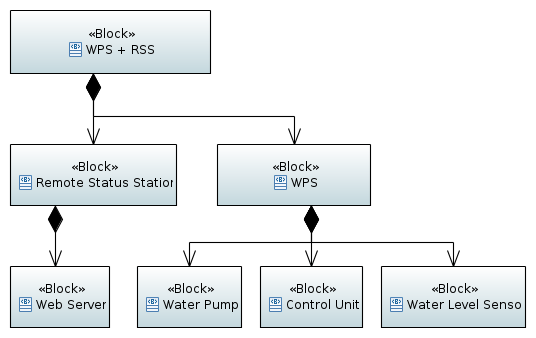
\includegraphics[width=300px]{../diagrams/system-structure.png}
  \caption{System Structure diagram}
  \label{fig:System Structure Diagram}
\end{figure}

Looking at the prototype's deployment diagram \ref{fig:deployment-diagram}, we can clearly see that, the output of the modeling, traces nicely to its implementation.
The grayed parts of the diagram don't make up the prototype. 

\begin{figure}[H]
  \centering
  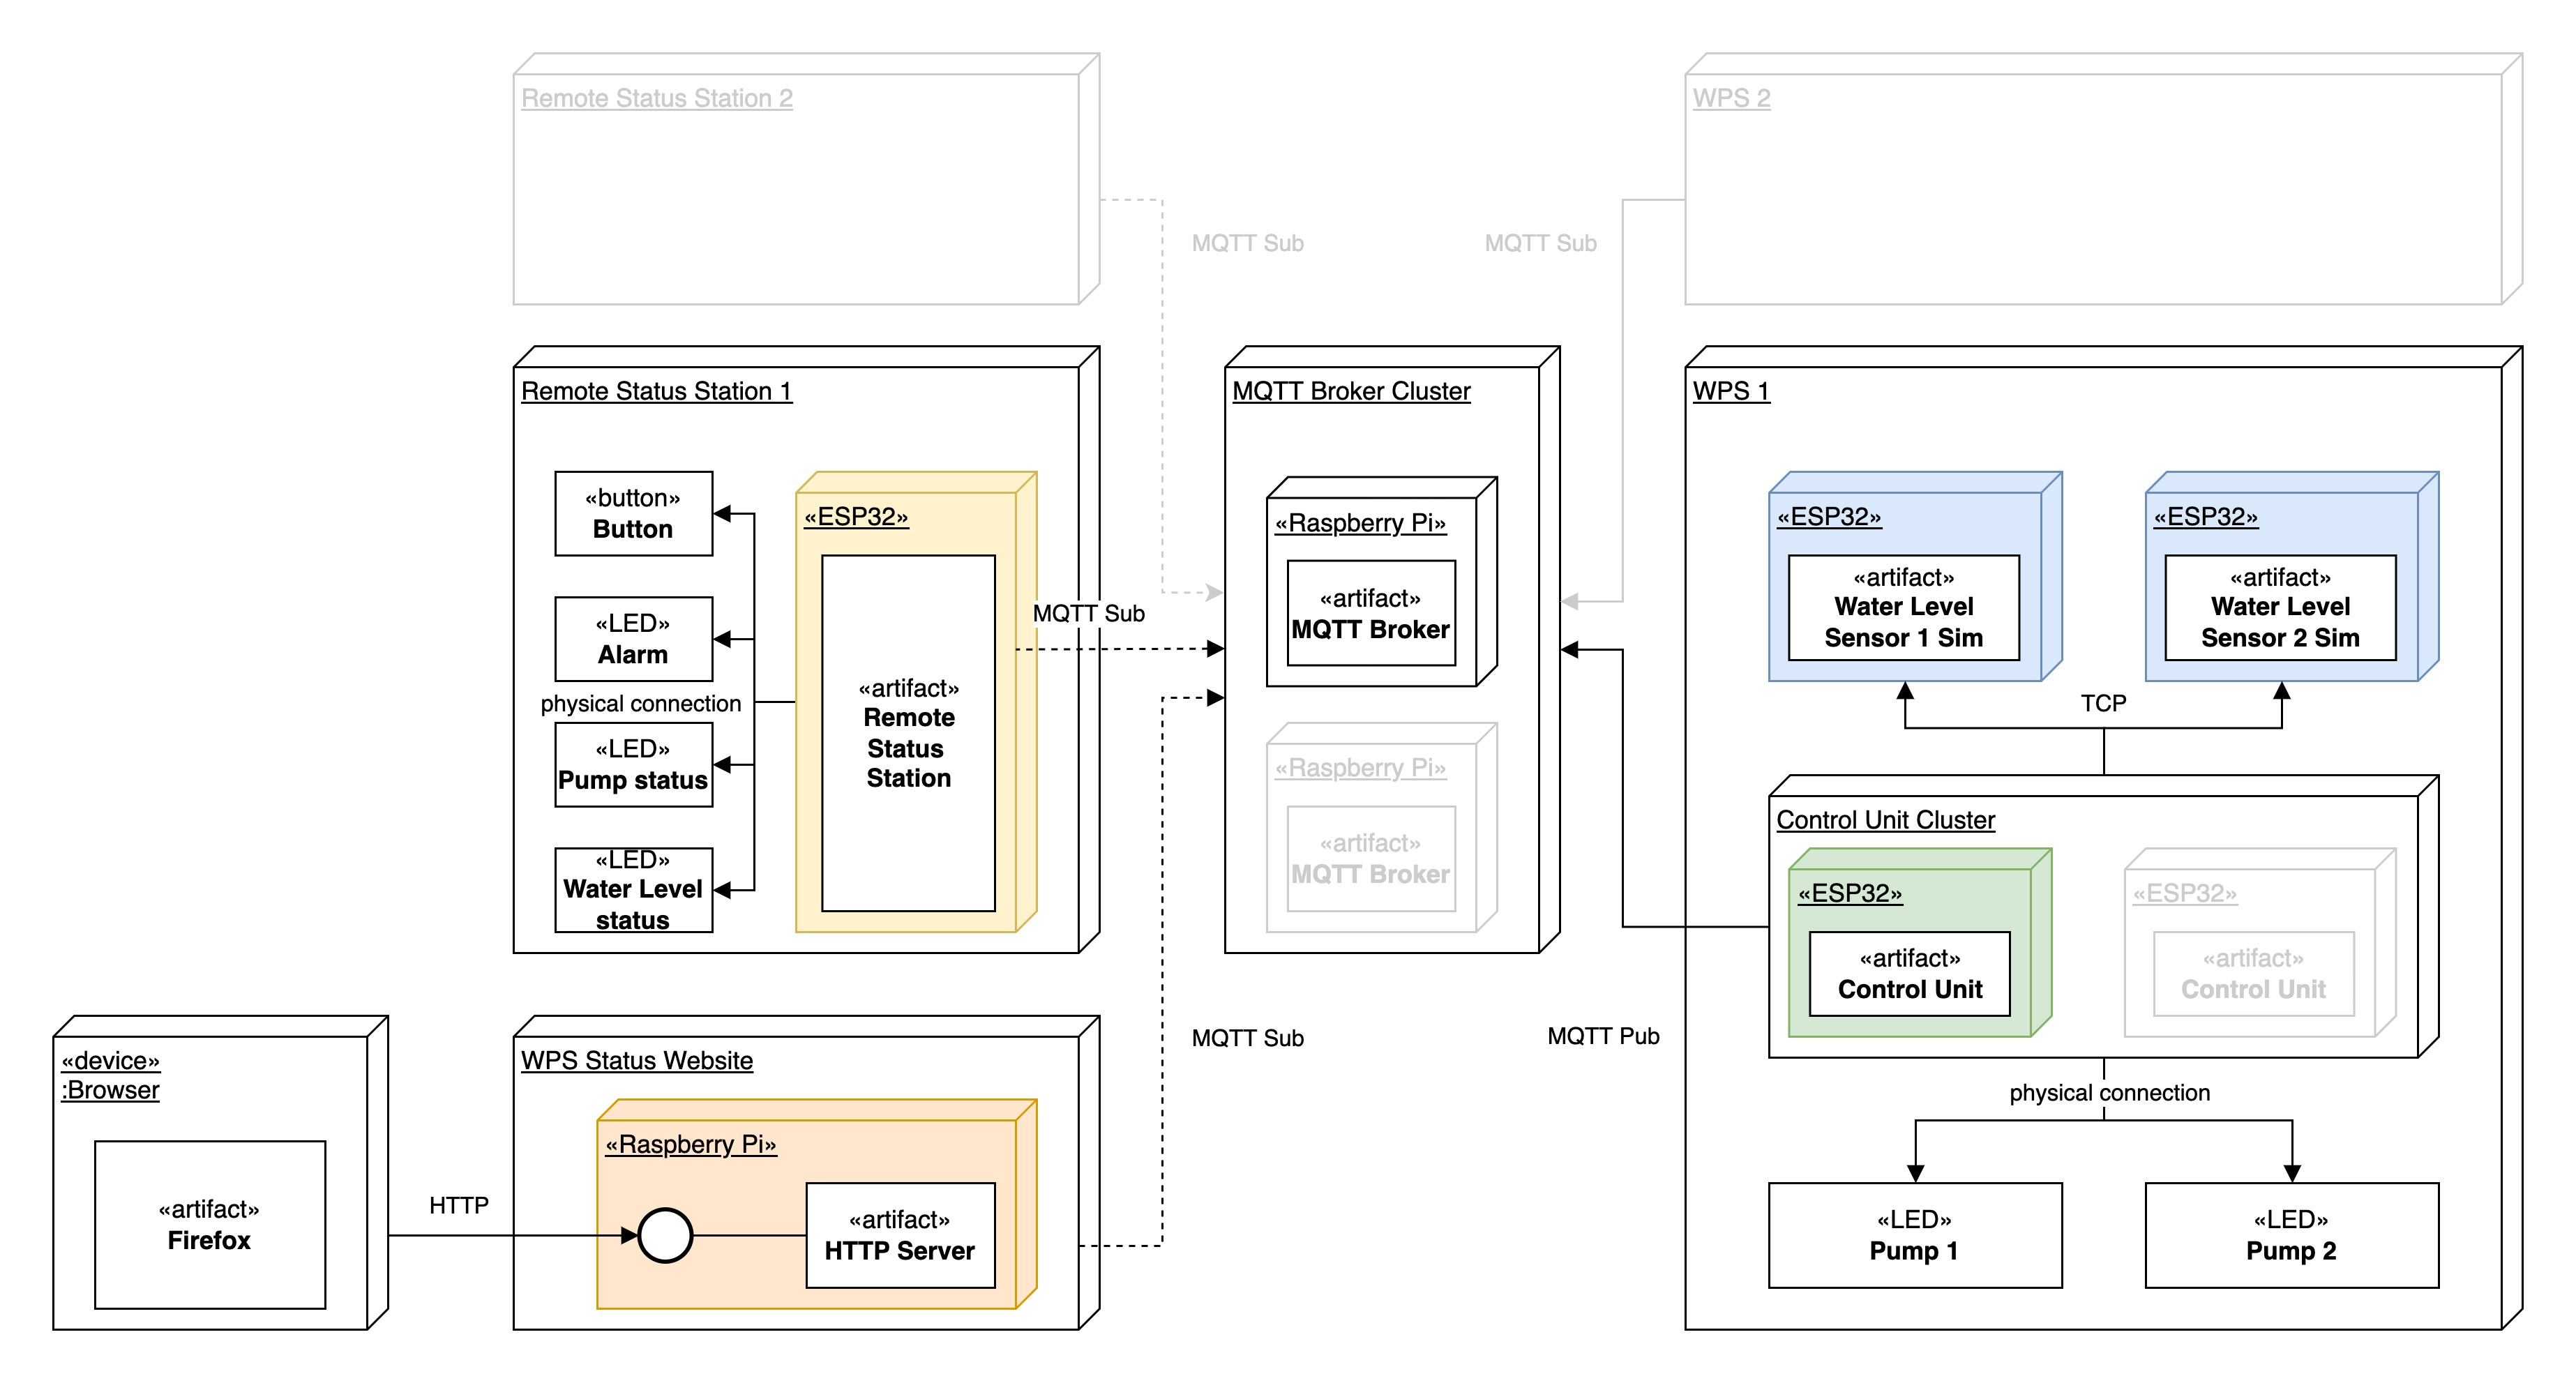
\includegraphics[width=\linewidth]{../diagrams/deployment-diagram.jpg}
  \caption{Prototype's deployment diagram}
  \label{fig:deployment-diagram}
\end{figure}

\newpage
%%%
\section{Implementation}

%%%
\subsection{CCSYA - Assembly}

The following code snippet in implemented on the Sensor Sim, as it was in the previous delivery. The only change was done on one of the comments that had a typo.

\begin{minted}[linenos]{gas}
.global getMask

getMask:    entry a1, 48
            movi a5, 0          # init increment
            mov a6, a2          # save inputed water level
            movi a2, 1          # init return value

loop: 
            addi a5, a5, 1      # increment by one
            beq a5, a6, end     # branch to 'end' if equal
            slli a2, a2, 1      # left shif by 1, i.e. 0001 -> 0010
            j loop              # jump to loop 

end:
            retw.n
\end{minted}

As an input, the code receives the position of the LED that needs to turn ON. So to ensure that only one of the LEDs is turned ON, we start with the value 1 (see line 6). This value in a byte is represented by \texttt{'0000 0001'}. From now on, we only shift the leftmost bit, one position at a time, until we reach the selected position.

The output is an 8-bit integer. If we have as output the decimal number \texttt{'16'}, and convert it to binary \texttt{´0000 1000´}, we can see that we want to turn ON the LED in the 4th position. The following code implements this logic. 

\begin{minted}{c}
// more code

  mask = getMask(level); // ASM code
  implementMask(mask);

// more code

void implementMask(int8_t mask)
{
  int8_t n_bit = 0;
  while (n_bit < MAX_LEVELS) {
    if (mask & 0x01) {
      digitalWrite(STATES[n_bit], HIGH);
    }
    else {
      digitalWrite(STATES[n_bit], LOW);
    }
    n_bit++;
    mask = mask >> 1;
  }
}
\end{minted}


%%%
\subsection{RTAES - Concorrency and Real Time Scheduling}

%%%
\subsubsection{Implementation of the Tasks and Concorrency control}

As a remainder, the following tasks are being run in a ESP-WROOM-32 on a single core:

\begin{itemize}
	\item  \textbf{Task 1}: Retrieve data from sensors (TCP Client);
	\item  \textbf{Task 2}: Process data and give instructions to pumps;
	\item  \textbf{Task 3}: Publish WPS status to MQTT broker (MQTT client).
\end{itemize}

\noindent
The creation of the tasks was achieved by using the \textbf{xTaskCreatePinnedToCore(...)} \cite{c1} function from the FreeRTOS API. The function \textbf{xTaskCreate(...)} was also available, but we wanted to ensure that the proposed tasks would run on the same core.

\begin{minted}{c}
xTaskCreatePinnedToCore(
                    requestSensorData,   /* Task function. */
                    "Task1",     /* name of task. */
                    10000,       /* Stack size of task */
                    NULL,        /* parameter of the task */
                    1,           /* priority of the task */
                    &Task1,      /* Task handle to keep track of created task */
                    0);          /* pin task to core 0 */  
\end{minted}

The access control to the critical section was done thanks to the use of a single semaphore: \texttt{xSemaphoreHandle xMutex;}.

%%%
\subsubsection{Real Time Scheduling}

It must be openly said that this part was the trickiest one.

To check in pratical terms, the results of the schedulability calculation done in the previous report, some changes needed to be added to the code.

Although the execution times for Task 2 look to be very close to the ones achieved in the calculations, the same doesn't apply for Task 1 and Task 3. This is partly the fault of communication latency. Both tasks need to request or send information using a wireless connection and the TCP/IP protocol.

Another problem was the method implemented to track the task's execution time. The granularity wasn't enough, especially for Task 2.

As a practical solution, we chose to update the values from the last report in a proportionally way.
 
\begin{table}[H]
    \caption{Theoretical values (left) and implemented values (right) in \textit{ms}:}
    \begin{minipage}{0.7\linewidth}
		\begin{table}[H]
		\begin{tabular}{lll}
		\textbf{Task} & \textbf{Ci} & \textbf{Ti} \\
		\textbf{1}    & 60         & 100           \\
		\textbf{2}    & 25         & 200           \\
		\textbf{3}    & 35         & 250          
		\end{tabular}
		\label{table:rt-1}
		\end{table}
    \end{minipage}%
    \begin{minipage}{.5\linewidth}
		\begin{table}[H]
		\begin{tabular}{lll}
		\textbf{Task} & \textbf{Ci} & \textbf{Ti} \\
		\textbf{1}    & 1200         & 2000           \\
		\textbf{2}    & 500         & 4000           \\
		\textbf{3}    & 700         & 5000          
		\end{tabular}
		\label{table:rt-2}
		\end{table}
    \end{minipage} 
\end{table}

The values on the right side were achieved by running the code in different situations. A closer look, shows that we incresed all values \textbf{x 20}.

To track the execution time we added the following code to each task:

\begin{minted}{c}
for (;;) {
    unsigned long start_time = millis();
    unsigned long finish_time;
    unsigned long duration;

    // Code -------------------

    finish_time = millis();      
    duration = finish_time - start_time;
    Serial.print("TASK N - Execution Time[ms]: ");
    Serial.println(duration); 
}
\end{minted}

\noindent
And here are some of the outputs:

\begin{minted}{bash}
TASK 3 - Duration[ms]: 40
TASK 1 - Duration[ms]: 917
TASK 2 - Duration[ms]: 475
TASK 1 - Duration[ms]: 658
TASK 1 - Duration[ms]: 754
TASK 3 - Duration[ms]: 770  < above WCET
TASK 2 - Duration[ms]: 476
TASK 1 - Duration[ms]: 649
TASK 1 - Duration[ms]: 799
TASK 3 - Duration[ms]: 29
TASK 2 - Duration[ms]: 477
TASK 1 - Duration[ms]: 176
TASK 1 - Duration[ms]: 997
TASK 2 - Duration[ms]: 481
TASK 1 - Duration[ms]: 187
TASK 3 - Duration[ms]: 157
TASK 1 - Duration[ms]: 990
TASK 2 - Duration[ms]: 475
TASK 1 - Duration[ms]: 1036
\end{minted}

It is important to state, that given the short execution time of Task 2, we needed to add a sleep function to increase it and so bring it closer to the values on the right side table \ref{table:rt-2}.

Also, to control that the tasks didn't extended beyond its deadline, we added the following code:

\begin{minted}{c}
long next_release = 5000 - duration; // 5 seconds deadline for Task 3
if (next_release > 0) {
    vTaskDelay(next_release / portTICK_PERIOD_MS);
} else {
    Serial.println("TRASK 3 - FAILED Deadline !!!");
}
\end{minted}

In some cases, Task 1 failed the deadline by a couple of milliseconds. This was because of the defined timeout value of 1 second for each TCP request (one request per sensor). When the two requests reached a timeout, we already had a 2-second execution time. Unfortunately, the library used for the TCP connection has a lower limit of 1 second for the timeout. 

We consciously chose not to fix this issue, mostly because a fix would mean a more extended increase of the values, beyond the x20, and when we have at least one sensor responding, the execution time are very close to the ones in the table \ref{table:rt-2}.

\begin{minted}{bash}
TASK 1 - Connection failed: 172.20.10.13
TASK 1 - Connection failed: 172.20.10.5
TASK 1 - Duration[ms]: 2009
TASK 1 - FAILED Deadline !!!
\end{minted}

%%%
\subsubsection{Concorrency}

In terms of concurrency and, as proposed in the last report, we identified as a critical section the read and write of a data structure that encapsulates the WPS status.

\begin{minted}{c}
typedef struct{
  volatile bool alert;
  volatile uint8_t id;
  volatile uint8_t curr_water_level;
  volatile uint8_t curr_pump1_status;
  volatile uint8_t curr_pump2_status;  
  volatile uint8_t curr_pump1_state;
  volatile uint8_t curr_pump2_state;
} WPS;
\end{minted}

The changes to the data structure WPS were made by accessing functions instead of accessing the values directly.

\begin{minted}{c}
void set_curr_pump2_status(uint8_t value) {
  xSemaphoreTake(xMutex, portMAX_DELAY);
  _wps.curr_pump2_status = value;
  xSemaphoreGive(xMutex);
}
\end{minted}

The status reads, were specially controlled during the publication of the WPS status to the MQTT broker.

\begin{minted}{c}
String getWpsStatus(){
    xSemaphoreTake(xMutex, portMAX_DELAY);
    String message = String(_wps.alert) + "," + String(_wps.id) + "," + String(_wps.curr_water_level) + "," + String(_wps.curr_pump1_status) + "," + String(_wps.curr_pump2_status);
    xSemaphoreGive(xMutex);
    return message;
}
\end{minted}

%%%
\subsection{COMCS - Communication}

- TCP pull strategy

- Arthur

%%%
\subsection{Prototype}

%%%
\subsubsection{Overview}

An overview of what was implemented in the prototype can be found in diagram \ref{fig:deployment-diagram}.

The cluster of MQTT brokers, or Control Units, were not implemented, as were the second WPS and the second RSS.
However, the system was developed to accommodate the future implementation of all the missing parts.

With a cluster of MQTT brokers, the producer (Control Units) and the consumers (Web server and RSS) would need to connect to all the available nodes and jump from one to the other if there were some type of failure.

The cluster of Control Units would be implemented by running both systems in parallel but only outputting one of the results. If the computations of both nodes differ, the implementation of a type of voting system needs to be implemented.

A second WPS is easily solved because for each system there must be one MQTT topic. This means one queue per WPS and a consumer subscription to each one of them.

\begin{figure}[H]
  \centering
  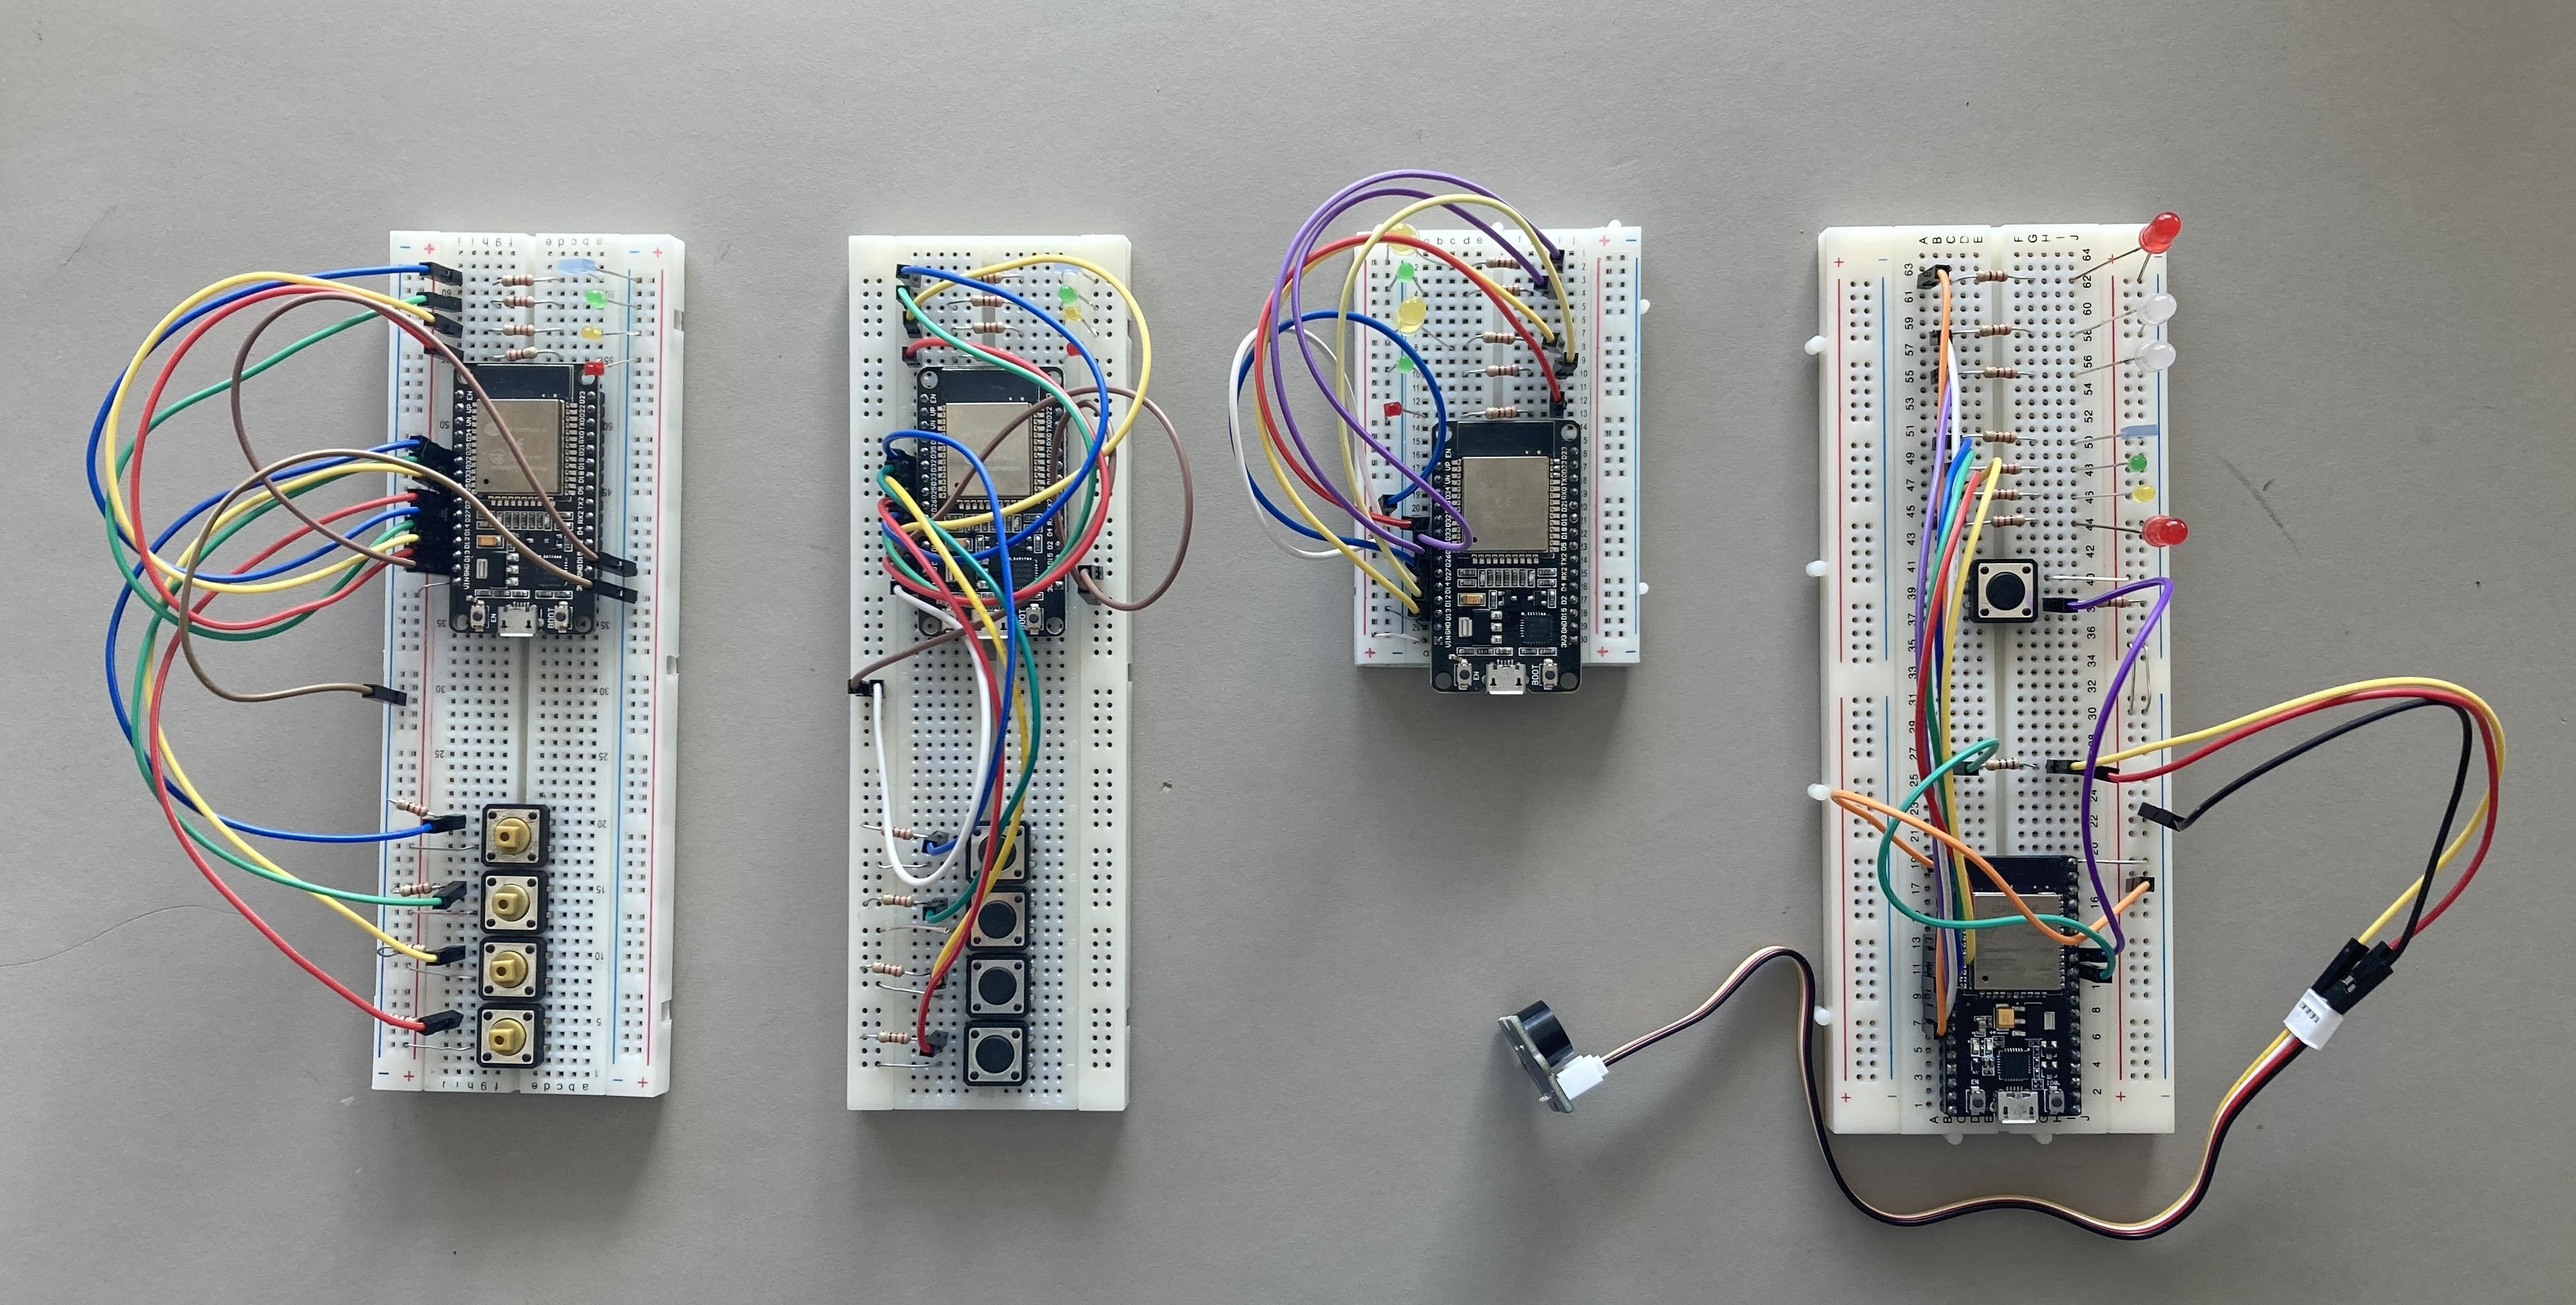
\includegraphics[width=\linewidth]{../diagrams/hardware.jpg}
  \caption{from left to right: Sensor 1, Sensor 2, Control Unit + Pumps, RSS}
  \label{fig:hardware}
\end{figure}

Below is a representation of the topological layout of the network that will be presented.

\begin{figure}[H]
  \centering
  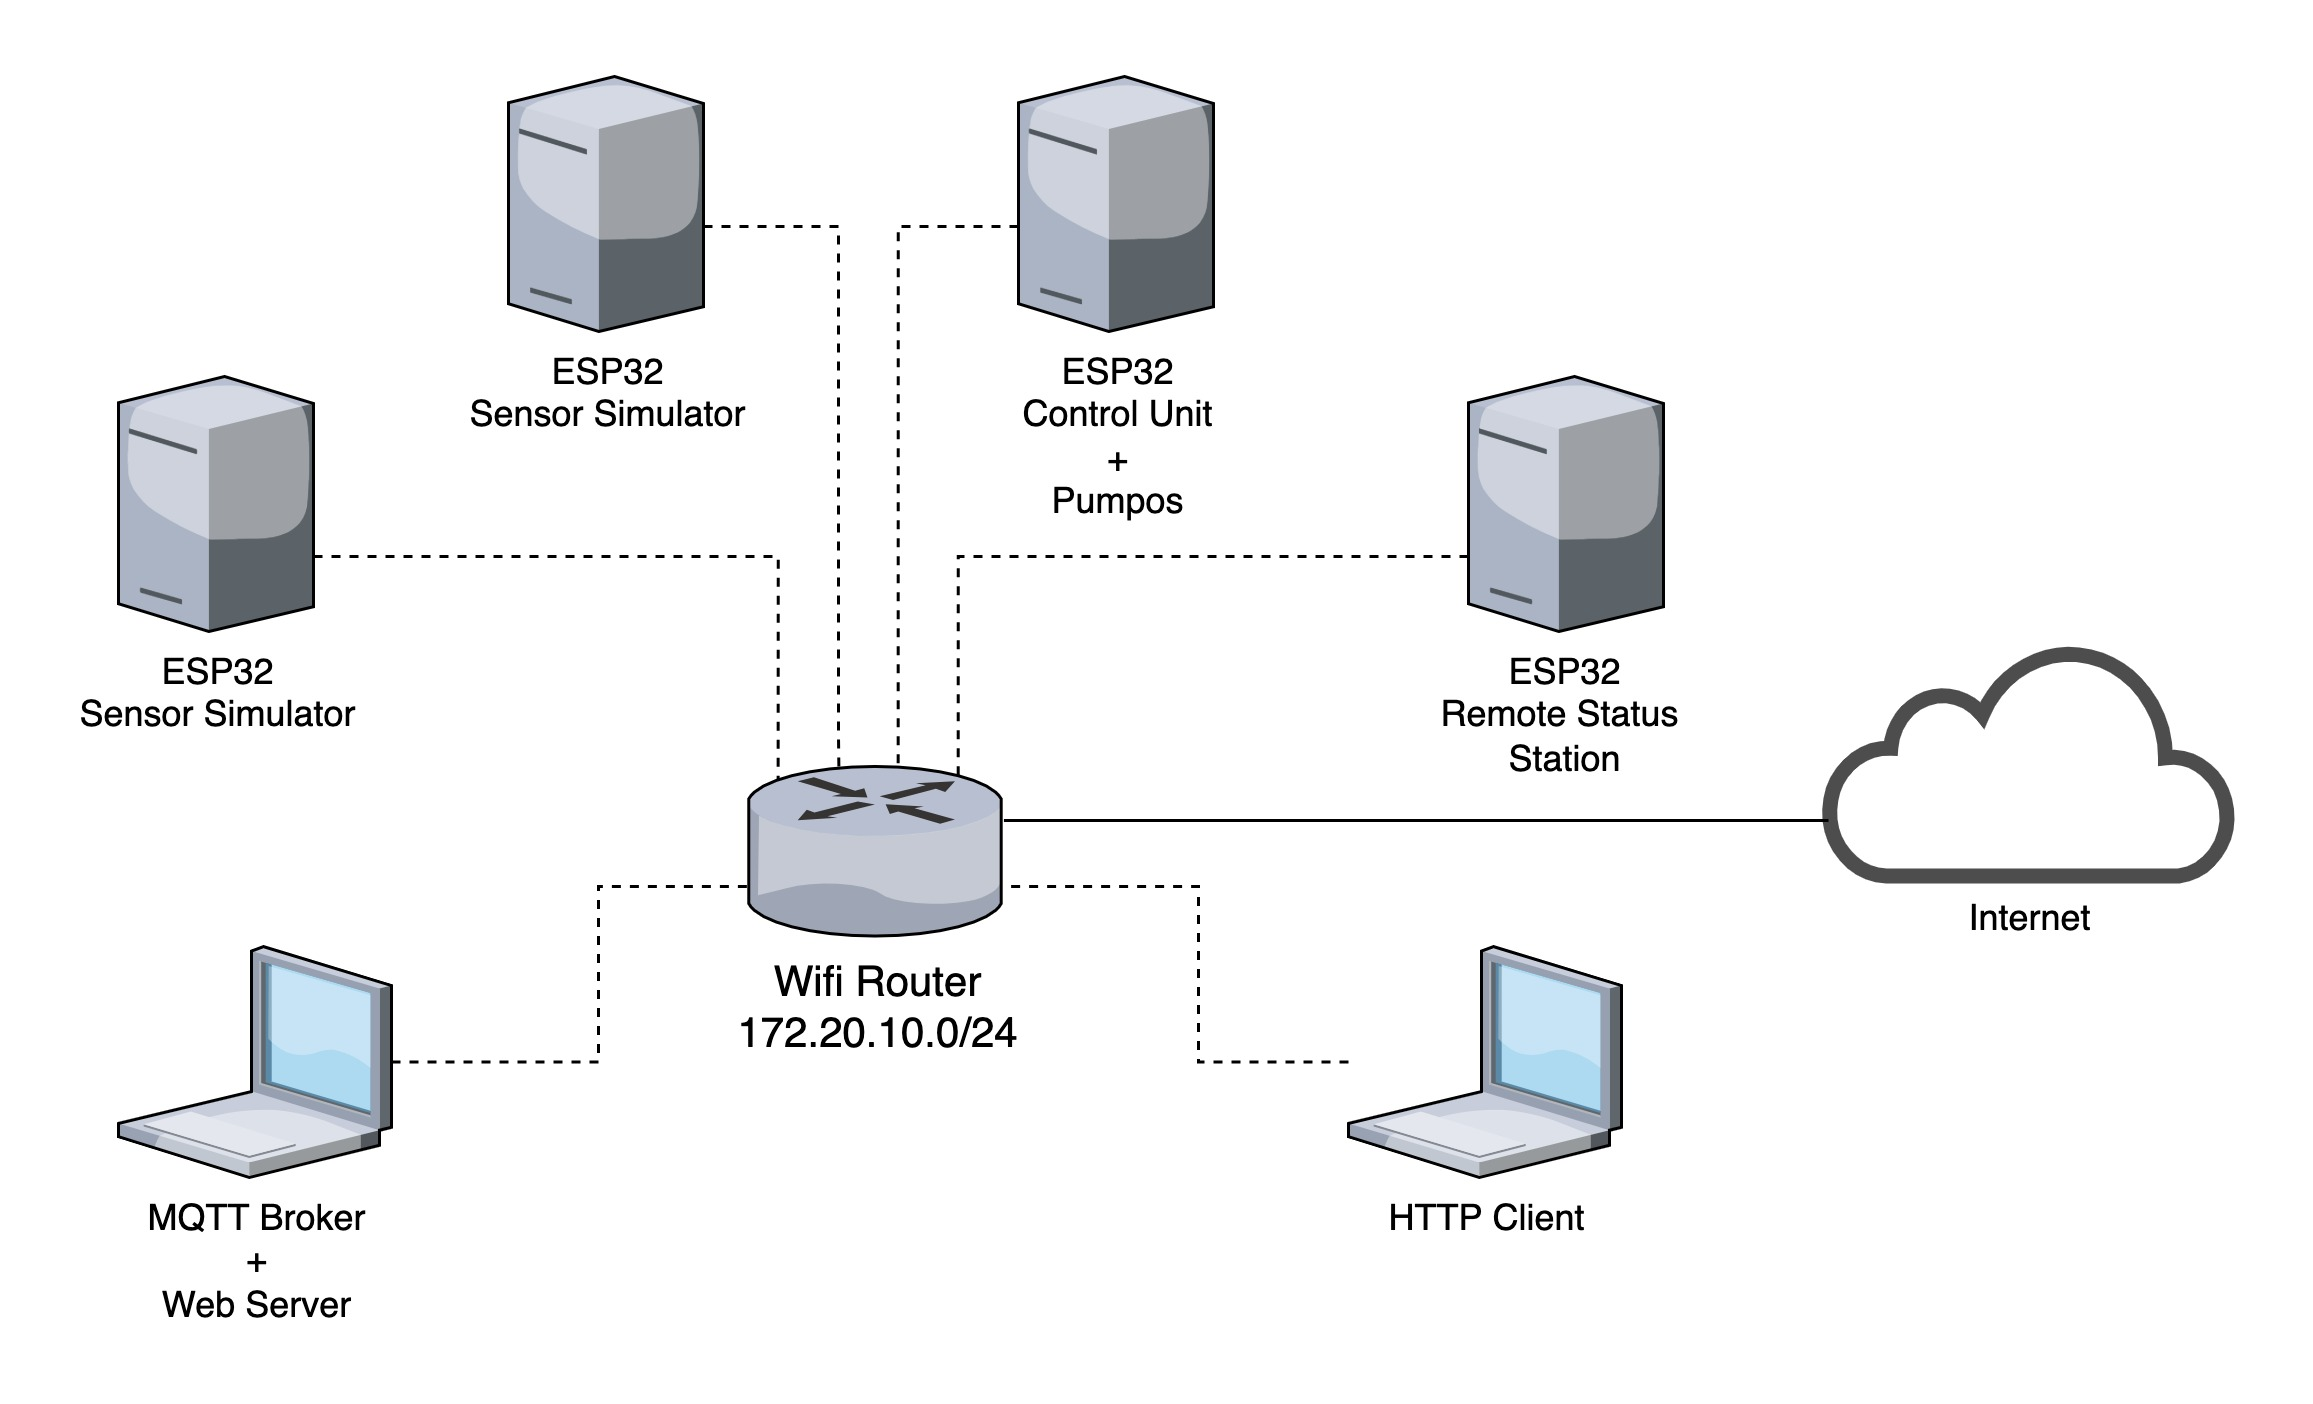
\includegraphics[width=300px]{../diagrams/network-diagram.jpg}
  \caption{Network diagram}
  \label{fig:network-diagram}
\end{figure}

%%%
\subsubsection{Control Unit}

The WPS will publish a message with its status, every 5 seconds.

Looking at the right tabel \ref{table:rt-2}, we can also notice that we are able to do 2 requests to the sensor (Task 1) for each computation of the systems behavior (Task 2). This gives us the possibility to recover from a communication failure when doing one of the two requests.

The main behavior of the system is summurized by all the requirements from SR-1.
\newline
\newline
\noindent
\textbf{Used hardware:}
\begin{itemize}
	\item ESP-32
	\item 1x alert LED
	\item 2x pump status LEDs
	\item 2x pump state LEDs (able or not to do some work)
\end{itemize}

%%%
\subsubsection{RSS}

The MQTT client in the RSS will, every second, query the broker for a new message. If no new message is available in the last 15 seconds, an alarm will be triggered. This means that the Control Unit, which publishes to the broker every 5 seconds, has three chances to recover from some communication failure. 

Although we are simulating only one WPS, subscribing to a second topic with the status of the second WPS is easily done.
\newline
\newline
\noindent
\textbf{Used hardware:}
\begin{itemize}
	\item ESP-32
	\item 1x buzzer module
	\item 1x button to stop buzzer
	\item 1x alert LED
	\item 2x pump status LEDs
	\item 4x water level LEDs
\end{itemize}

%%%
\subsubsection{Sensor}
\noindent
\textbf{Used hardware:}
\begin{itemize}
	\item ESP-32
	\item 4x water level buttons
	\item 4x water level LEDs
\end{itemize}

\subsubsection{Web Server}

The Web Server follows the same logic as the RSS. It consumes the same topics made available by the broker.

We ponder another approach, where the Web server would query the RSS for the WPS status. This solution would give more responsibilities to a critical system (RSS) and make all the implementation more complex and unnecessary.

%%%
\section{Team Work}

Because of thoughtful analysis during the first delivery, the solution analysis gave us a list of very decoupled subsystems. This enabled us to split the work in a more organized way, as soon as the communication method was defined.

The drafting of the reports was done in cooperation, giving us the opportunity to share some particular knowledge of each subsystem.

In a more concrete way, we create a common repository on Bitbucket, where each main change in the code base is done by creating a Pull Request. This made both of us aware of the work as a whole.

In conclusion, the teamwork ran smoothly, mainly because of an initial good analysis of the system requirements, and also because of the focus on the academic objectives of this work.

%%%%%%%%%%%%%%%%%%%%%
\newpage
\begin{thebibliography}{8}

\bibitem{c1}
 Espressif FreeRTOS API: {\url{https://docs.espressif.com/projects/esp-idf/en/v4.3/esp32/api-reference/system/freertos.html}}

\end{thebibliography}

\end{document}
